\subsection{DNA methylation data} \label{dna-methylation-data-sect}
DNA methylation is a well studied chemical modification of DNA, which occurs when a methyl group is attached to a DNA nucleotide. It is associated with diverse biological processes of direct clinical relevance, including gene and transposon silencing, X-chromosome inactivation, and  genomic imprinting \citep{Li1993, Mohandas1981}. In mammals,  methylation is observed almost exclusively on cytosine residues in the context of CpG dinucleotides (\ie C followed by G, where p stands for the phosphate group linking C and G). DNA methylation is said to be a true \emph{epigenetic modification}, since its mechanism of inheritance during the cell cycle is well established \citep{Law2010}. 

Due to the increased vulnerability of the 5-methylcytosines to randomly deaminate to thymine, most of the genome is depleted from CpG dinucleotides \citep{Scarano1967}, except from small regions termed \emph{CpG islands} \citep{Bird2002}. A CpG island (CGI) is a sequence of at least 200 bp with a greater number of CpG sites than expected from its GC content. These regions are often GC rich, typically undermethylated, and are found upstream of many mammalian genes \citep{Law2010}. 

Bisulphite treatment \citep{Frommer1992} followed by NGS can be used to measure the methylation level of the genomic DNA at a single-nucleotide resolution, and is termed Whole-Genome Bisulphite Sequencing (WGBS). Sodium bisulphite efficiently deaminates unmethylated cytosines to uracils, and leaves the 5-Methylcytosines unchanged. Uracils are read as thymines by DNA polymerase, thus when amplifying the data during PCR (Polymerase Chain Reaction), the unmethylated cytosines appear as thymines \citep{Krueger2012}. Reads are then aligned to a reference genome allowing changes of C to T during the mapping procedure. 
The outline of the bisulphite treatment of a sample DNA sequence is shown in \emph{Figure \ref{bisulphite-pic}}.
\begin{figure}[!ht]
	\begin{center}
 		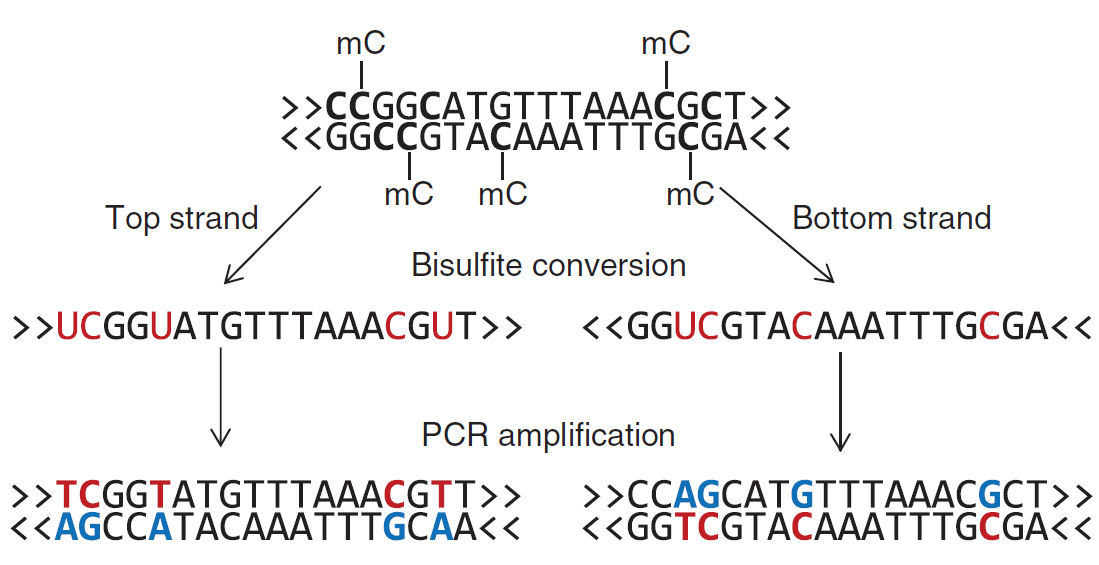
\includegraphics[scale = 0.4]{images/bis-treatment.png}
		\caption{\emph{Outline of the bisulphite treatment and subsequent PCR amplification of a sample DNA sequence. Unmethylated cytosines are deaminated to uracils by bisulphite, while 5-Methylcytosines are resistant to conversion \citep{Krueger2012}.}}
		\label{bisulphite-pic}
	\end{center}
\end{figure} 

In WGBS experiments, the DNA molecules often originate from distinct cells, as a consequence, the methylation state of a particular cytosine may be different across DNA molecules. Hence, in the context of WGBS experiments the methylation of a particular cytosine is described as \emph{methylation level}, which is the fraction of the molecules in the sample containing 5-Methylcytosine at the specific genomic locus \citep{Schultz2012}. \emph{Read coverage} is the average number of times a CpG site is read during the sequencing process, and this depends on the sequencing depth.

\cite{Meissner2005} developed a technique, termed Reduced Representation Bisulfite Sequencing (RRBS), for analyzing the genome-wide methylation profiles efficiently, at lower cost and with greater coverage of CpG dense regions. This method, combines bisulphite treatment and restriction enzymes, such as MspI, to generate a 'reduced representation' of the genome of a strain, tissue or cell type which have a high CpG content \citep{Meissner2005}. 

%For the purpose of this project, RRBS data from the H1-hESC and K562 cells will be analysed. Both datasets were generated by the Myers Lab at the HudsonAlpha Institute for Biotechnology. 